\chapter{Recursividade}\label{cap10}

\epigraph{Recursive. adj. See RECURSIVE.}{Stan Kelly-Bootie --- The
  Devil's DP Dictionary}

\section{Motivação}

Tanto em matemática, quanto na ciência da computação, diversas
operações são definidas recursivamente, isto é, alguns valores
iniciais para esta operação são dados e os demais são obtidos
aplicando-se uma ou mais regras sucessivamente. Um exemplo de função
recursiva é a definição do fatorial, apresentada abaixo:

\[
\begin{array}{lcl}
0! & = & 1\\
n! & = & n \times (n - 1)!
\end{array}
\]

Como valor inicial, temos que o fatorial de $0$ é $1$ e, demais
valores são obtidos pela segunda equação da definição.

De certa forma, provas por indução possuem uma estrutura similar a
definições recursivas: apresenta-se provas de fatos elementares (casos
base) e usa-se uma regra (passo indutivo) para mostrar que o fato em
questão é válido para elementos diferentes dos considerados nos casos
base. Neste capítulo, veremos como a indução é utilizada para
demonstrar propriedades sobre definições recursivas.

\section{Funções Recursivas}

Existem diversas maneiras de se definir funções. Podemos definir uma
função usando uma expressão que caracteriza a relação entre o domíno e
sua imagem (método usualmente utilizado na matemática). Outra maneira
de se definir uma função é através do uso de composição, que permite a
definição de funções utilizando definições prévias. Esta forma de
definir funções é o mais próximo do que idealmente deve ser feito em
computação, visto que fornece o mais elevado nível de abstração,  o
de composição de interfaces. Existe, ainda uma terceira forma de se definir uma função:
utilizando recursão. Como um primeiro exemplo,
considere a seguinte função $f : \mathbb{N} \to \mathbb{N}$ definida
como
\[
\left\{
\begin{array}{lcl}
  f(0) & = & 1 \\
  f(n) & = & 2n + f(n - 1)\\
\end{array}
\right .
\]
Note que esta definição especifica um valor inicial para $f$, $f(0) =
1$ e os demais valores são obtidos a partir de valores ``anteriores''
desta função. Como exemplo, considere o cálculo de $f(5)$, apresentado
abaixo:
\[
\begin{array}{lc}
f(5) & = \\
2.5 + f(4) & = \\
10 + (2.4 + f(3)) & = \\
10 + (8 + (2.3 + f(2))) & = \\
 10 + (8 + (6 + 2.2 + f(1))) & = \\
10 + (8 + (6 + (4 + (2.1 + f(0))))) & = \\
10 + (8 + (6 + (4 + (2 + 1)))) & = \\
31
\end{array}
\]
Apesar de simples compreensão, o uso de funções recursivas possui o
inconveniente de que o cálculo desta para valores elevados do domínio
pode consumir muito tempo. Considere calcular $f(2000)$. Este cálculo
ocasionaria $2000$ chamadas recursivas. Porém, muitas vezes, podemos
encontrar uma função $g$, equivalente a $f$, sem
recursividade. Existem diversas técnicas para solucionar este tipo de
problema e apresentaremos a mais simples destas baseada em indução matemática.
Inicialmente, montamos uma pequena tabela de valores para $f$:
\[
\begin{array}{|c|c|}
  \hline
  n & f(n) \\ \hline
  0 &  1 \\
  1 &  3 \\
  2 &  7 \\
  3 & 13 \\
  4 & 21 \\
  5 & 31 \\
  6 & 43 \\ \hline
\end{array}
\]
Após pensar um pouco, podemos conjecturar que a função
\[
g(n) = n (n+1) + 1
\]
é equivalente a $f$, uma vez que esta possui os mesmos valores que
$f$, conforme tabela abaixo:
\[
\begin{array}{|c|c|c|}
  \hline
  n & f(n) & g(n)\\ \hline
  0 &  1  & 1 \\
  1 &  3  & 3 \\
  2 &  7  & 7 \\
  3 & 13 & 13 \\
  4 & 21 & 21 \\
  5 & 31 & 31 \\
  6 & 43 & 43\\ \hline
\end{array}
\]
Porém, somente construir e verificar esta tabela para alguns valores
não é suficiente para mostrar que $f(n) = n(n+1) + 1$. Para isso,
devemos provar que:
\[
\forall n. n\in\mathbb{N} \to f(n) = n(n+1) + 1
\]
que pode ser provado por indução matemática, conforme apresentado no
teorema seguinte.

\begin{Theorem}
Seja $f(n)$ uma função definida como:
\[
\left\{
\begin{array}{lcl}
  f(0) & = & 1 \\
  f(n) & = & 2n + f(n - 1)\\
\end{array}
\right .
\]
então $f(n) = n(n+1) + 1$.
\end{Theorem}
\begin{proof}
\verb| |\\
\begin{enumerate}
  \item[\ ]Caso base ($n = 0$): Temos que $f(0) = 1 = 0(0 +1) + 1$,
    conforme requerido.
  \item[\ ]Passo indutivo: Suponha $n\in\mathbb{N}$ arbitrário e que
    $f(n) = n(n+1) + 1$. Temos:
   \[
      \begin{array}{lcl}
      f(n+1) & = \\
      2 (n+1) + f(n) & = & \text{pela definição de }f(n)\\
      2(n+1) + n(n+1) + 1 & = & \text{pela hipótese de indução}\\
      (n+1)[(n+1) + 1] +1
      \end{array}
   \]
   Logo, $f(n+1) = (n+1)[(n+1) + 1] + 1$ conforme requerido.
\end{enumerate}
\end{proof}

De maneira geral, podemos obter uma fórmula fechada (isto é, sem
recursividade) para uma função recursiva $f(n)$ usando os seguintes
passos:
\begin{enumerate}
  \item Construir uma tabela contendo alguns valores da função $f(n)$.
  \item ``Adivinhar'', a partir da tabela construída no passo
    anterior, qual função não recursiva produz os mesmos resultados
    para os valores da tabela.
  \item Provar, usando indução matemática, que a fórmula fechada
    encontrada é realmente equivalente a função em questão.
\end{enumerate}
A seguir, mostraremos mais exemplo desta técnica encontrando uma
fórmula fechada para a seguinte função recursiva.

\[
\left\{
\begin{array}{lcl}
    f(0) & = & 0\\
    f(n) & = & 2f(n - 1) + 1
\end{array}
\right.
\]
Inicialmente, construiremos uma tabela contendo alguns valores de
$f(n)$:
\[
\begin{array}{|c|c|}
  \hline
  n & f(n) \\ \hline
  0 &  0 \\
  1 &  1 \\
  2 &  3 \\
  3 &  7 \\
  4 & 15 \\
  5 & 31\\
  6 & 63 \\ \hline
\end{array}
\]
Se observarmos os valores da tabela, podemos perceber que estes são
próximos de potências perfeitas de $2$, logo, podemos conjecturar que
a fórmula fechada para $f(n)$ é $2^n - 1$. Constataremos este fato
provando por indução.
\begin{Theorem}\label{thmhanoi}
Seja $f(n)$ a função definida como
\[
\left\{
\begin{array}{lcl}
    f(0) & = & 0\\
    f(n) & = & 2f(n - 1) + 1
\end{array}
\right.
\]
então $f(n) = 2^n - 1$.
\end{Theorem}
\begin{proof}
\verb| |\\
\begin{enumerate}
  \item[\ ]Caso base: Para $n = 0$, temos $f(0) = 0 = 1 - 1 = 2^0 - 1$.
  \item[\ ]Passo indutivo: Suponha $n\in\mathbb{N}$ arbitrário e que
    $f(n) = 2^n - 1$. Temos que:
\[
\begin{array}{lcl}
    f(n + 1) & = & \\
    2f(n) + 1 & = & \\
    2(2^n - 1) + 1 & = & \{\text{pela hipótese de indução}\}\\
    2^{n+1} - 2 + 1 & = &\\
    2^{n+1} - 1
\end{array}
\]
Logo, $f(n + 1) = 2^{n + 1} - 1$.
\end{enumerate}
\end{proof}

\subsection{Conjunto Potência, Recursivamente}

No capítulo \ref{cap5}, apresentamos a definição do conjunto potência
(ou conjunto das partes) de um conjunto $A$:
\[\mathcal{P}(A) =\{X\,|\,X\subseteq A\}\]
É fácil mostrar que $|\mathcal{P}(A)| = 2^n$ se $|A| = n$, usando o
princípio multiplicativo (veja no capítulo \ref{cap6}).

Porém, como provar este resultado usando indução? Pode-se argumentar que basta
utilizar indução sobre o tamanho do conjunto. Logo, no caso base, para
$n = 0$, consideramos o conjunto vazio e obtemos $\mathcal{P}(\emptyset)=\{\emptyset\}$.

No caso indutivo, devemos considerar o cálculo do conjunto potência de
um conjunto $A$ com pelo menos um elemento. Isto é:
\[
A = B \cup \{a\}\,\,\,a\not\in B
\]

Essas observações levam a seguinte função recursiva que, a partir de
um conjunto qualquer, produz o conjunto potência deste.

\[
\left\{
\begin{array}{lcl}
\mathcal{P}(\emptyset) & = & \{\emptyset\}\\
\mathcal{P}(B \cup \{a\}) & = & \mathcal{P}(B)\cup \{X \cup
\{a\}\,|\,X \in \mathcal{P}(B)\}\,\,\,\,\text{em que }a\not\in B
\end{array}
\right.
\]
Observe que o cálculo do conjunto potência inclui o elemento $a$ em
cada um dos subconjuntos de $B$. Evidentemente, como $\mathcal{P}(B)$
e $\{X \cup\{a\}\,|\,X \in \mathcal{P}(B)\}$ são disjuntos e cada um
destes possui $2^n$ elementos (pela hipótese de indução), temos que
$|\mathcal{P}(A)| = 2^{n + 1}$. A demonstração deste fato é
apresentada a seguir.

\begin{Theorem}
Para todo $A$, se $|A| = n$ então $|\mathcal{P}(A)|=2^{n}$.
\end{Theorem}
\begin{proof}
\verb| |\\
\begin{enumerate}
  \item[\ ]Caso base ($n = 0$): Neste caso, temos que $A =
    \emptyset$. Logo, $|P(\emptyset)| = |\{\emptyset\}| = 1 = 2^0$,
    conforme requerido.
  \item[\ ]Passo indutivo: Suponha $n \in\mathbb{N}$ arbitrário e que
    $|B| = n$ e $|\mathcal{P}(B)| = 2^n$. Suponha $a$ arbitrário tal
    que $a\not\in B$ e que $A = B \cup {a}$. Seja $X = \{Y \cup
    \{a\}\,|\,Y \in \mathcal{P}(B)\}$. É óbvio que $|X| = 2^n$. Como
    $\mathcal{P}(A) = \mathcal{P}(B) \cup X$, temos que
    $|\mathcal{P}(A)| = |\mathcal{P}(B)| + |X| = 2^n + 2^n = 2^{n + 1}$.
\end{enumerate}
\end{proof}


\subsection{A Sequência de Fibonacci}

A sequência de Fibonacci é uma sequência de números inteiros em que os
dois primeiros números são $0$ e $1$ e os demais são obtidos somando
os dois termos anteriores, isto é:
\[
0,1,1,2,3,5,8,13,21, 34, 55, 89, 144, 233, 377, …
\]
Evidentemente podemos representar o $n$-ésimo termo desta sequência
pela seguinte função recursiva:
\[
\left\{
\begin{array}{lcl}
F(0) & = & 0 \\
F(1) & = & 1 \\
F(n) & = & F(n - 1) + F(n - 2)
\end{array}
\right.
\]
Como exemplo de uso desta função, considere o seguinte cálculo de $F(5)$:
\[
\begin{array}{lc}
F(5) & = \\
\underbrace{F(4) + F(3)}_{F(5)} & = \\
\underbrace{F(3) + F(2)}_{F(4)} + \underbrace{F(2) + F(1)}_{F(3)} & = \\
\underbrace{F(2) + F(1)}_{F(3)} + \underbrace{F(1) + F(0)}_{F(2)} +
\underbrace{F(1) + F(0)}_{F(2)} + 1 & = \\
\underbrace{F(1) + F(0)}_{F(2)} + 1 + 1 + 0 + 1 + 0 + 1& =\\
1 + 0 + 1 + 1 + 0 + 1 + 0 + 1& = \\
5
\end{array}
\]
Evidentemente, que um algoritmo baseado nesta definição para calcular
$F(n)$ será extremamente ineficiente. Desta forma, devemos procurar
uma fórmula fechada para a sequência de Fibonacci de maneira que
possamos calcular um elemento desta sequência sem usar recursão ou
algum tipo de repetição.

Apesar de existir uma técnica para encontrar fórmulas fechadas para
funções recursivas como a para a sequência de Fibonacci, o uso desta
foge ao escopo deste texto. Ao invés disso, vamos apresentar a fórmula
fechada para $F(n)$ e provar que esta realmente corresponde a
definição recursiva apresentada.

\begin{Theorem}
Seja $F(n)$ o $n$-ésimo termo da sequência de Fibonacci. Então,
\[
F(n) = \dfrac{\left(\dfrac{1 + \sqrt{5}}{2}\right)^n - \left(\dfrac{1 - \sqrt{5}}{2}\right)^n}{\sqrt{5}}
\]
\end{Theorem}
\begin{proof}
Suponha $n\in\mathbb{N}$ arbitrário. Suponha que para todo
$k\in\mathbb{N}$, $k < n$, temos que:
\[
F(k) = \dfrac{\left(\dfrac{1 + \sqrt{5}}{2}\right)^k - \left(\dfrac{1 - \sqrt{5}}{2}\right)^k}{\sqrt{5}}
\]
 Considere os seguintes casos:
\begin{enumerate}
  \item Caso $n = 0$: Temos que:
  \[
\begin{array}{lc}
    F(0) & =\\
    0     & = \\
    \dfrac{0}{\sqrt{5}} & = \\
    \dfrac{1 - 1}{\sqrt{5}} & = \\
    \dfrac{\left(\dfrac{1 + \sqrt{5}}{2}\right)^0 - \left(\dfrac{1 - \sqrt{5}}{2}\right)^0}{\sqrt{5}}
\end{array}
  \]
  conforme requerido.
  \item Caso $n = 1$: Temos que:
  \[
\begin{array}{lc}
    F(1) & =\\
    1     & = \\
    \dfrac{\sqrt{5}}{\sqrt{5}} & = \\
    \dfrac{\dfrac{2\sqrt{5}}{2}}{\sqrt{5}} & = \\
    \dfrac{\dfrac{\sqrt{5} + \sqrt{5} + 1 - 1}{2}}{\sqrt{5}} & = \\
    \dfrac{\left(\dfrac{1 + \sqrt{5}}{2}\right)^1 - \left(\dfrac{1 - \sqrt{5}}{2}\right)^1}{\sqrt{5}}
\end{array}
  \]
  conforme requerido.
  \item Caso $n\geq 2$: Temos que:
\[
\begin{array}{lcl}
F(n) & = \\
F(n - 1) + F(n - 2) & = & \{\text{pela def. de }F(n)\}\\
\dfrac{\left(\dfrac{1 + \sqrt{5}}{2}\right)^{n - 1} - \left(\dfrac{1 -
      \sqrt{5}}{2}\right)^{n - 1}}{\sqrt{5}} +
\dfrac{\left(\dfrac{1 + \sqrt{5}}{2}\right)^{n - 2} - \left(\dfrac{1 -
      \sqrt{5}}{2}\right)^{n - 2}}{\sqrt{5}} & = \\
\dfrac{\left(\dfrac{1 + \sqrt{5}}{2}\right)^{n - 2}\left(1 + \dfrac{1
      + \sqrt{5}}{2}\right) - \left(\dfrac{1 - \sqrt{5}}{2}\right)^{n - 2}\left(1 + \dfrac{1
      - \sqrt{5}}{2}\right)}{\sqrt{5}} & = \\
\dfrac{\left(\dfrac{1 + \sqrt{5}}{2}\right)^{n - 2}\left(\dfrac{1
      + \sqrt{5}}{2}\right)^2 - \left(\dfrac{1 - \sqrt{5}}{2}\right)^{n - 2}\left(\dfrac{1
      - \sqrt{5}}{2}\right)^2}{\sqrt{5}} & = \\
\dfrac{\left(\dfrac{1 + \sqrt{5}}{2}\right)^n - \left(\dfrac{1 - \sqrt{5}}{2}\right)^n}{\sqrt{5}}
\end{array}
\]
\end{enumerate}
conforme requerido.
\end{proof}

Note que nesta prova usamos o fato de que os números $\frac{1 +
  \sqrt{5}}{2}$ e $\frac{1 -\sqrt{5}}{2}$ são soluções da seguinte
equação: $x^2 = x + 1$, isto é, são números que se somarmos um a eles,
produziremos este número elevado a segunda potência. Além disso,
perceba que esta
prova só é possível utilizando indução forte, pois precisamos que a
hipótese seja válida não apenas para o antecessor de $n$, $ n - 1$,
mas também para $n - 2$. É útil o leitor tentar provar este teorema
usando indução convencional e perceber onde não é possível continuar
com a demonstração.

\section{Problemas Recursivos}

A seguir apresentamos alguns problemas clássicos e como estes podem
ser modelados utilizando funções recursivas. Além dessa modelagem,
apresentaremos como obter uma fórmula fechada equivalente a função apresentada.

\subsection{As Torres de Hanói}

As torres de Hanói é um quebra-cabeça inventado por um matemático
francês, Édouard Lucas em 1833.  Este quebra-cabeça consiste de uma
torre contendo uma quantidade $n\in\mathbb{N}$ de discos, inicialmente
empilhados em ordem decrescente de tamanho. A figura abaixo, apresenta
a configuração inicial deste quebra-cabeças:

\begin{figure}[h!]
  \centering
      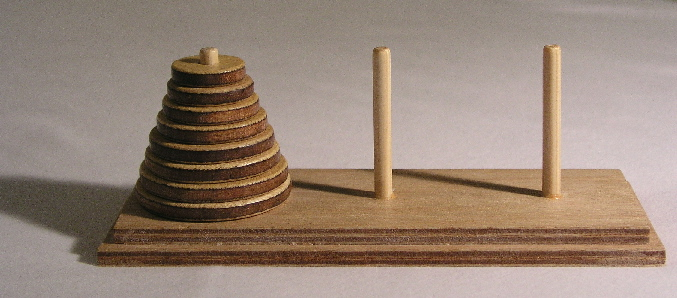
\includegraphics[width=0.5\textwidth]{imagens/torredehanoi.jpg}
 \end{figure}
O objetivo deste jogo é transferir todos os discos de um pino para
outro movendo apenas um disco de cada vez e nunca colocando um disco
maior em cima de um menor.

Apesar de simples, não é óbvio que este quebra-cabeças possui
solução. Após pensar um pouco, podemos perceber que este de fato,
sempre possui solução. Porém, qual será a melhor? Isto é, é possível
solucionar este problema fazendo o menor número de movimentos?

Para chegar a resposta para esta pergunta, devemos primeiro introduzir
algumas notações. Chamaremos de $T(n)$ o número de movimentos
necessários para solucionar o quebra cabeças contendo $n$ discos.

É bastante fácil ver que $T(0) = 0$ e que $T(1) = 1$. A figura
seguinte, mostra passo a passo, a solução para $n = 2$.\\

\begin{figure}[H]
  \centering
      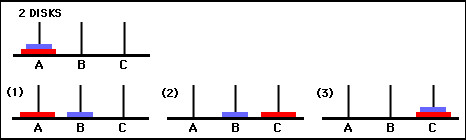
\includegraphics[width=0.5\textwidth]{imagens/hanoi2.jpg}
 \end{figure}

Para $n = 3$, temos: \\

\begin{figure}[h!]
  \centering
      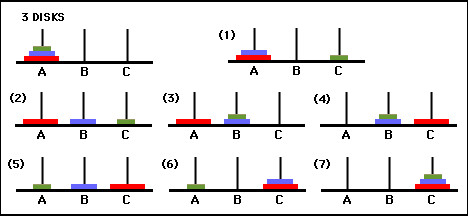
\includegraphics[width=0.5\textwidth]{imagens/hanoi3.jpg}
 \end{figure}

Com isso, temos a seguinte tabela de valores iniciais de $T(n)$:

\[
\begin{array}{|c|c|}
  \hline
  n & T(n)\\ \hline
  0  & 0 \\
  1  & 1 \\
  2 & 3 \\
  3 & 7\\
  \hline
\end{array}
\]

Agora, que fizemos alguns experimentos com este problema, vamos mudar
nossa perspectiva: ao invés de tentar pensar em como resolver este
problema para casos específicos, vamos tentar
generalizá-lo. Observando a figura para a solução com 3 discos,
podemos perceber que o problema para $n = 3$ é resolvido da seguinte
maneira:
\begin{itemize}
  \item Mova $n - 1$ discos do pino $A$ para o pino $B$.
  \item Mova o disco $n$ do pino $A$ para o pino $C$.
  \item Mova $n - 1$ discos do pino $C$ para o pino $C$.
\end{itemize}
Como, para mover $n - 1$ discos de um pino para outro, precisamos de $T(n
-1)$ movimentos, no total precisamos de
\[
T(n - 1) + T(n - 1) + 1 = 2T(n - 1) + 1
\]
para solucionar um quebra-cabeças de tamanho $n$. Assim, temos que o
número mínimo de movimentos para a solução deste problema é dado pela
seguinte função recursiva:
\[
\left\{
\begin{array}{lcl}
T(0) & = & 0 \\
T(n) & = & 2 T(n - 1) + 1
\end{array}
\right.
\]
Mas será que esta função reflete os resultados que obtivemos
solucionando o problema? Vamos fazer os cálculos para $n = 3$:
\[
\begin{array}{lc}
T(3) & = \\
2 T(2) + 1 & = \\
2(2T(1) + 1) + 1 & =\\
2(2(2T(0) + 1) + 1) + 1 & = \\
2(2(2.0 + 1) + 1) + 1 & = \\
7
\end{array}
\]
conforme requerido. Como vimos anteriormente, funções recursivas são
usualmente ineficientes para o cálculo manual. Logo, é uma boa prática
encontrarmos uma fórmula fechada para a função em questão. Porém, já
encontramos esta fórmula no teorema \ref{thmhanoi}.


\subsection{O Problema da Pizzaria}

Suponha que em um fim de semana você tenha ido a uma pizzaria que
possuía a seguinte promoção:

\begin{quote}
``O cliente que conseguir descobrir o número máximo de pedaços que pode
ser obtido ao se fazer $n \in \mathbb{N}$ cortes em uma pizza, não a pagará.''
\end{quote}

Então, como pode-se comer uma pizza de graça? Novamente, vamos seguir
a estratégia utilizada no exemplo anterior. Primeiro, vamos chamar de
$T(n)$ o número de fatias obtidas após fazermos o $n$-ésimo corte. É
bem fácil perceber que $T(0) = 1$, visto que se não fizermos nenhum
corte, temos uma fatia (a pizza inteira). Usando um raciocínio
parecido, temos que $T(1) = 2$, visto que ao fazermos um corte, iremos
dividir a pizza em dois pedaços. Porém, quantos pedaços obtemos ao
fazer o $3^o$ corte? A intuição nos diz que devemos obter $T(3) = 6$,
porém, conforme mostrado na próxima figura, isso não é bem verdade...

\begin{figure}[H]
  \centering
      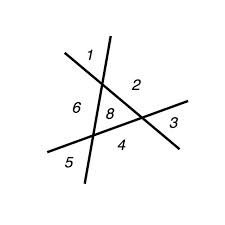
\includegraphics[width=0.5\textwidth]{imagens/plane.jpg}
 \end{figure}

Note que obtemos um número maior de pedaços fazendo com que o
$n$-ésimo corte intercepte todos os cortes anteriores. Com isso,
aumentamos o número total de fatias em $n$ pedaços, isto é, $T(3) = 4
+ 3 = 7$, em que $4 = T(2)$. Desta forma, podemos conjecturar que
$T(n)$ é a seguinte função recursiva:

\[
\left\{
\begin{array}{lcl}
  T(0) & = & 1 \\
  T(n) & = & T(n - 1) + n
\end{array}
\right.
\]

Note que ao calcularmos alguns valores de $T(n)$, podemos notar que
este nada mais é que a soma dos $n$ primeiros números naturais somados
com 1, conforme expandido abaixo:

\[
\begin{array}{lcl}
T(n) & = & T(n - 1) + n \\
       & = & (T(n - 2) + (n - 1)) + n\\
       & = & ( (T(n - 3) + (n - 2)) + (n - 1)) + n\\
       &  & \vdots\\
       & = & T(0) + 1 + 2 + ... + (n -2) + (n - 1) + n\\
       & = & 1 + 1 + 2 + ... + (n -2) + (n - 1) + n\\
       & = & 1 + \sum_{k = 1}^nk
\end{array}
\]
Pode-se mostrar por indução que $\sum_{k = 1}^n =
\frac{n(n+1)}{2}$. Logo, temos que $T(n)$ é dado por:
\[
T(n) = \frac{n(n+1)}{2} + 1
\]
Realmente esta fórmula corresponde a função $T(n)$, conforme provamos
no teorema a seguir.

\begin{Theorem}
Seja $T(n)$ a função definida como:
\[
\left\{
\begin{array}{lcl}
  T(0) & = & 1 \\
  T(n) & = & T(n - 1) + n
\end{array}
\right.
\]
então, $T(n) = \frac{n(n+1)}{2} + 1$.
\end{Theorem}
\begin{proof}
\verb| |\\
\begin{enumerate}
  \item[\ ]Caso base ($n = 0$): Temos que $T(0) = \frac{0(0 + 1)}{2} +
    1$, conforme requerido.
  \item[\ ]Passo indutivo: Suponha $n\in\mathbb{N}$ arbitrário e que
    $T(n) = \frac{n(n+1)}{2} + 1$. Temos que:
   \[
\begin{array}{lcl}
T(n + 1) & = \\
T(n) + (n + 1) & = & \{\text{pela def. de }T(n)\}\\
\frac{n(n+1)}{2} + 1 + (n + 1) & = & \{\text{pela hipótese de
  indução}\}\\
\frac{n(n + 1) + 2(n+1)}{2} & = & \\
\frac{(n + 1)(n + 2)}{2}
\end{array}
   \]
conforme requerido.
\end{enumerate}
\end{proof}

\subsection{Preenchendo um Tabuleiro de Xadrez}

Considere seguinte quebra-cabeça: preencher um tabuleiro $2^n \times 2^n$, $n
\in \mathbb{N}$, $n\geq 1$, com peças em formato de ``L'' como a
apresentada abaixo:
\begin{figure}[H]
  \centering
      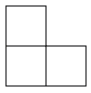
\includegraphics[width=0.15\textwidth]{imagens/tromino.png}
 \end{figure}
de maneira que apenas uma posição do tabuleiro não seja ocupada por
estas peças. Abaixo apresentamos a solução deste quebra-cabeças para
um tabuleiro de $2^3\times 2^3$:
\begin{figure}[H]
  \centering
      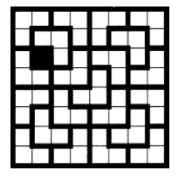
\includegraphics[width=0.35\textwidth]{imagens/tab5.png}
 \end{figure}
em que a posição não ocupada por peças é a que está em ``preto''. A
questão é como resolver este quebra-cabeças para um valor qualquer de
$n \geq 1$?

É fácil ver pela figura abaixo que o quebra-cabeça é obviamente
solúvel para $n = 1$.
\begin{figure}[H]
  \centering
      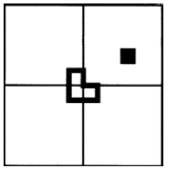
\includegraphics[width=0.35\textwidth]{imagens/tab1.png}
 \end{figure}
Mas, como solucionar este quebra-cabeças para um $n > 1$? O ponto
principal para solucionar este problema para $n > 1$ é observar que um
tabuleiro $2^{n + 1} \times 2^{n + 1}$ é formado por $4$ tabuleiros de
$2^n\times 2^n$. Logo, podemos resolver o quebra-cabeça para um
tabuleiro de $2^{n + 1} \times 2^{n + 1}$ a partir das 4 soluções para
tabuleiros de $2^n\times 2^n$. A chave para combinar as soluções de
cada um dos ``pedaços'' dos quebra cabeças é deixar a posição não
preenchida de cada um destes na extremidade em que esta faz junção
com os outros tabuleiros de mesmo tamanho. Como são 4 tabuleiros de
tamanho $2^n\times 2^n$, haverão 4 posições não preenchidas,
permitindo assim o encaixe de mais uma peça em L, completando a
solução do quebra-cabeça.

A descrição informal acima apresentada, mostra como resolver este
quebra-cabeça, isto é, fornece um algoritmo recursivo para o problema
em questão. Além disso, esta mesma descrição é exatamente a estrutura
de uma prova por indução que mostra que este problema é solúvel para
todo $n \geq 1$. Isto não é uma mera coincidência. Normalmente, provas
por indução possuem a mesma estrutura de algoritmos recursivos.

\begin{Theorem}
Para todo $n \geq 1$, temos que todo tabuleiro de $2^n \times 2^n$
pode ser preenchido por peças em forma de ``L'' de maneira que somente
uma posição do tabuleiro não seja ocupada por uma destas peças.
\end{Theorem}
\begin{proof}
A prova será por indução sobre $n$.
\begin{enumerate}
  \item Caso base ($n = 1$). Imediato. Basta ocupar o tabuleiro com
    uma peça em forma de ``L''.
  \item Passo indutivo. Suponha $n \in \mathbb{N}$ arbitrário e que
    todo tabuleiro de $2^n \times 2^n$ possa ser preenchido de forma que
    apenas uma posição não esteja ocupada. Como um tabuleiro de $2^{n
      + 1} \times 2^{n + 1}$ é formado por 4 tabuleiros de $2^n\times
    2^n$, pela hipótese de indução, estes 4 tabuleiros podem ser
    preenchidos de maneira que uma posição destes não seja
    preenchida. Deixando a posição vazia destes tabuleiros de
    $2^n\times 2^n$ no ponto de junção destes tabuleiros, podemos
    formar a solução para o tabuleiro de $2^{n+1}\times 2^{n+1}$
    acrescentando uma peça, deixando apenas uma posição livre,
    completando assim o quebra-cabeça.
\end{enumerate}
\end{proof}

\section{Exercícios}
\begin{enumerate}
	\item Encontre uma f\'ormula fechada (sem recursividade) equivalente a cada uma das fun\c{c}\~oes recursivas a seguir
		  e prove que a f\'ormula encontrada \'e equivalente a fun\c{c}\~ao em quest\~ao.
	\begin{enumerate}
		\item
				$\left\{
					\begin{array}{l}
						T(0) = 0 \\
						T(n) = 2T(n - 1) + n
					\end{array}
			    \right .$

		\item
				$\left\{
					\begin{array}{l}
						T(0) = 2 \\
						T(n) = (T(n - 1))^{2}
					\end{array}
			    \right .$

		\item
				$\left\{
					\begin{array}{l}
						T(0) = 2 \\
						T(n) = 2T(n - 1) + n
					\end{array}
			    \right .$

		\item
				$\left\{
					\begin{array}{l}
						T(1) = 1 \\
						T(n) = \frac{T(n-1)}{1 + T(n - 1)}
					\end{array}
			    \right .$
               \item
                            $\left\{
					\begin{array}{l}
						T(1) = \frac{1}{4} \\
						T(2) = \frac{1}{8}\\
                                                T(n) =
                                                \frac{T(n-1)T(n-2)}{2T(n-2)
                                                - T(n-1)}
					\end{array}
			    \right .$
	\end{enumerate}
	\item Seja $F(n)$ o $n$-\'esimo termo da sequ\^encia de Fibonacci, definida como:
	\[
		\left\{
			\begin{array}{lcl}
				F(0) & = & 0\\
				F(1) & = & 1 \\
				F(n) & = & F(n - 1) + F(n - 2)
			\end{array}
		\right.
	\]
	Prove os seguintes fatos sobre a sequ\^encia de Fibonacci.
	\begin{enumerate}
		\item $\sum_{i=0}^{n}F(i) = F(n + 2) - 1$
		\item $\sum_{i=0}^{n}F(2i + 1) = F(2n + 2)$
		\item $\sum_{i=0}^{n}(F(i))^{2} = F(n)F(n+1)$
		\item Prove que para todo $n\in\mathbb{N}$, $F(n) < 2^n$.
	\end{enumerate}
        \item Seja $A$ um conjunto. Representamos por
          $\mathcal{P}_{2}(A)$ o conjunto de todos os subconjuntos de
          $A$ que contém $2$ elementos. Prove que para todo conjunto
          $A$, se $|A| = n$, então $|\mathcal{P}_{2}(A)| = \frac{n (n - 1)}{2}$.
\end{enumerate}

\section{Notas Bibliográficas}

Recursividade e sua relação com a indução matemática é um tema
presente em todo texto de matemática discreta. O foco do capítulo
atual foi o uso de indução matemática para demonstrar fórmulas
fechadas equivalentes a funções recursivas. Alguns dos exemplos deste
capítulo foram retirados de \cite{Graham94}.